\documentclass[]{article}
\usepackage{lmodern}
\usepackage{amssymb,amsmath}
\usepackage{ifxetex,ifluatex}
\usepackage{fixltx2e} % provides \textsubscript
\ifnum 0\ifxetex 1\fi\ifluatex 1\fi=0 % if pdftex
  \usepackage[T1]{fontenc}
  \usepackage[utf8]{inputenc}
\else % if luatex or xelatex
  \ifxetex
    \usepackage{mathspec}
  \else
    \usepackage{fontspec}
  \fi
  \defaultfontfeatures{Ligatures=TeX,Scale=MatchLowercase}
\fi
% use upquote if available, for straight quotes in verbatim environments
\IfFileExists{upquote.sty}{\usepackage{upquote}}{}
% use microtype if available
\IfFileExists{microtype.sty}{%
\usepackage{microtype}
\UseMicrotypeSet[protrusion]{basicmath} % disable protrusion for tt fonts
}{}
\usepackage[margin=1in]{geometry}
\usepackage{hyperref}
\hypersetup{unicode=true,
            pdftitle={Final Report},
            pdfauthor={Isaac Slagel and Jack Welsh},
            pdfborder={0 0 0},
            breaklinks=true}
\urlstyle{same}  % don't use monospace font for urls
\usepackage{color}
\usepackage{fancyvrb}
\newcommand{\VerbBar}{|}
\newcommand{\VERB}{\Verb[commandchars=\\\{\}]}
\DefineVerbatimEnvironment{Highlighting}{Verbatim}{commandchars=\\\{\}}
% Add ',fontsize=\small' for more characters per line
\usepackage{framed}
\definecolor{shadecolor}{RGB}{248,248,248}
\newenvironment{Shaded}{\begin{snugshade}}{\end{snugshade}}
\newcommand{\KeywordTok}[1]{\textcolor[rgb]{0.13,0.29,0.53}{\textbf{#1}}}
\newcommand{\DataTypeTok}[1]{\textcolor[rgb]{0.13,0.29,0.53}{#1}}
\newcommand{\DecValTok}[1]{\textcolor[rgb]{0.00,0.00,0.81}{#1}}
\newcommand{\BaseNTok}[1]{\textcolor[rgb]{0.00,0.00,0.81}{#1}}
\newcommand{\FloatTok}[1]{\textcolor[rgb]{0.00,0.00,0.81}{#1}}
\newcommand{\ConstantTok}[1]{\textcolor[rgb]{0.00,0.00,0.00}{#1}}
\newcommand{\CharTok}[1]{\textcolor[rgb]{0.31,0.60,0.02}{#1}}
\newcommand{\SpecialCharTok}[1]{\textcolor[rgb]{0.00,0.00,0.00}{#1}}
\newcommand{\StringTok}[1]{\textcolor[rgb]{0.31,0.60,0.02}{#1}}
\newcommand{\VerbatimStringTok}[1]{\textcolor[rgb]{0.31,0.60,0.02}{#1}}
\newcommand{\SpecialStringTok}[1]{\textcolor[rgb]{0.31,0.60,0.02}{#1}}
\newcommand{\ImportTok}[1]{#1}
\newcommand{\CommentTok}[1]{\textcolor[rgb]{0.56,0.35,0.01}{\textit{#1}}}
\newcommand{\DocumentationTok}[1]{\textcolor[rgb]{0.56,0.35,0.01}{\textbf{\textit{#1}}}}
\newcommand{\AnnotationTok}[1]{\textcolor[rgb]{0.56,0.35,0.01}{\textbf{\textit{#1}}}}
\newcommand{\CommentVarTok}[1]{\textcolor[rgb]{0.56,0.35,0.01}{\textbf{\textit{#1}}}}
\newcommand{\OtherTok}[1]{\textcolor[rgb]{0.56,0.35,0.01}{#1}}
\newcommand{\FunctionTok}[1]{\textcolor[rgb]{0.00,0.00,0.00}{#1}}
\newcommand{\VariableTok}[1]{\textcolor[rgb]{0.00,0.00,0.00}{#1}}
\newcommand{\ControlFlowTok}[1]{\textcolor[rgb]{0.13,0.29,0.53}{\textbf{#1}}}
\newcommand{\OperatorTok}[1]{\textcolor[rgb]{0.81,0.36,0.00}{\textbf{#1}}}
\newcommand{\BuiltInTok}[1]{#1}
\newcommand{\ExtensionTok}[1]{#1}
\newcommand{\PreprocessorTok}[1]{\textcolor[rgb]{0.56,0.35,0.01}{\textit{#1}}}
\newcommand{\AttributeTok}[1]{\textcolor[rgb]{0.77,0.63,0.00}{#1}}
\newcommand{\RegionMarkerTok}[1]{#1}
\newcommand{\InformationTok}[1]{\textcolor[rgb]{0.56,0.35,0.01}{\textbf{\textit{#1}}}}
\newcommand{\WarningTok}[1]{\textcolor[rgb]{0.56,0.35,0.01}{\textbf{\textit{#1}}}}
\newcommand{\AlertTok}[1]{\textcolor[rgb]{0.94,0.16,0.16}{#1}}
\newcommand{\ErrorTok}[1]{\textcolor[rgb]{0.64,0.00,0.00}{\textbf{#1}}}
\newcommand{\NormalTok}[1]{#1}
\usepackage{graphicx,grffile}
\makeatletter
\def\maxwidth{\ifdim\Gin@nat@width>\linewidth\linewidth\else\Gin@nat@width\fi}
\def\maxheight{\ifdim\Gin@nat@height>\textheight\textheight\else\Gin@nat@height\fi}
\makeatother
% Scale images if necessary, so that they will not overflow the page
% margins by default, and it is still possible to overwrite the defaults
% using explicit options in \includegraphics[width, height, ...]{}
\setkeys{Gin}{width=\maxwidth,height=\maxheight,keepaspectratio}
\IfFileExists{parskip.sty}{%
\usepackage{parskip}
}{% else
\setlength{\parindent}{0pt}
\setlength{\parskip}{6pt plus 2pt minus 1pt}
}
\setlength{\emergencystretch}{3em}  % prevent overfull lines
\providecommand{\tightlist}{%
  \setlength{\itemsep}{0pt}\setlength{\parskip}{0pt}}
\setcounter{secnumdepth}{0}
% Redefines (sub)paragraphs to behave more like sections
\ifx\paragraph\undefined\else
\let\oldparagraph\paragraph
\renewcommand{\paragraph}[1]{\oldparagraph{#1}\mbox{}}
\fi
\ifx\subparagraph\undefined\else
\let\oldsubparagraph\subparagraph
\renewcommand{\subparagraph}[1]{\oldsubparagraph{#1}\mbox{}}
\fi

%%% Use protect on footnotes to avoid problems with footnotes in titles
\let\rmarkdownfootnote\footnote%
\def\footnote{\protect\rmarkdownfootnote}

%%% Change title format to be more compact
\usepackage{titling}

% Create subtitle command for use in maketitle
\providecommand{\subtitle}[1]{
  \posttitle{
    \begin{center}\large#1\end{center}
    }
}

\setlength{\droptitle}{-2em}

  \title{Final Report}
    \pretitle{\vspace{\droptitle}\centering\huge}
  \posttitle{\par}
    \author{Isaac Slagel and Jack Welsh}
    \preauthor{\centering\large\emph}
  \postauthor{\par}
    \date{}
    \predate{}\postdate{}
  
\usepackage{booktabs}
\usepackage{longtable}
\usepackage{array}
\usepackage{multirow}
\usepackage{wrapfig}
\usepackage{float}
\usepackage{colortbl}
\usepackage{pdflscape}
\usepackage{tabu}
\usepackage{threeparttable}
\usepackage{threeparttablex}
\usepackage[normalem]{ulem}
\usepackage{makecell}
\usepackage{xcolor}

\usepackage{dcolumn} \usepackage{float}

\begin{document}
\maketitle

\subsection{Introduction}\label{introduction}

According to an ASPCA estimate, over 6.5 millions animals enter a
shelter system every year. (Cite 1). After entering the shelter system
animals are either rehabilitated and sent to homes or euthanized. Animal
shelters, while running mostly on revenue from donations and adoption
fees, routinely run into perminant defieciets and must be supported with
money from local governments (Cite 2). Knowing more about the outcomes
of animals from these shelters could help us minimize the percent of
animals that need to be euthanized. Further, by identifying which
animals are less likely to be adopted, we can help shelters allocate
resources to minimize the time these animals spend in the shelter
system.

Our research looks into animal shelters in the Dallas area using a
dataset provided by the city of Dallas on dallasopendata.com. This data
includes information about every animal that has been brought into an
animal shelter in the Dallas area. There are 61634 individual animals in
this dataset with with information about when and where the animal was
found, the health of the animal on arrival, and whether the animal was
adopted, euthinized or transfered.

Recent research on animal shelters have consistantly shown that outcomes
for pitbulls are consistantly worse than other dog breeds (Patronek \&
Crowe 2018, Lepper et al 2002). We are interested in seeing if these
this trends exist in the Dallas animal shelter system.

\subsection{Materials and Methods}\label{materials-and-methods}

We accessed our data from the Dallas Open Data website. This website
contains many public datasets, including
\href{https://www.dallasopendata.com/City-Services/Dallas-Animal-Shelter-Data/7h2m-3um5}{animal
shelter records}. Anyone can request an access key to this dataset and
then download it. We downloaded the data, selected the variables of
interest to us, and created a .csv file in the CreateDataset.Rmd file.
Our dataset is saved as adoptions.csv. The initial variables from this
dataset are described below in Table 1.

\begin{table}[!h]

\caption{\label{tab:variable table}Description of Variables}
\centering
\resizebox{\linewidth}{!}{
\fontsize{12}{14}\selectfont
\begin{tabular}{llll}
\toprule
Variable Name & Variable Role & Variable Type & Description\\
\midrule
\rowcolor{gray!6}  out\_dead & response & bianary & Whether or not an animal was dead at the outcome\\
days\_in\_shelter & response & time & The number of days an animal spent in the animal shelter\\
\rowcolor{gray!6}  summer & explanatory & bianary & Whether or not an animal had its outcome in May-Sept\\
pitbull & explanatory & bianary & Whether or not a dog was a pitbull\\
\rowcolor{gray!6}  chip\_status & explanatory & bianary & Whether or not an animal had a scannable chip\\
contagious & potential confounder & bianary & Whether or not an animal was described as 'contagious' at intake\\
\rowcolor{gray!6}  treatable & potential confounder & bianary & Whether or not an animal was described as 'treatable' at intake\\
\bottomrule
\end{tabular}}
\end{table}

We used the imported data described in Table 1 to create a fleet of
indicator variables: \texttt{adopted}, \texttt{chip\_status},
\texttt{summer}, \texttt{treatable\_intake}, \texttt{adopted},
\texttt{dead}. These indicator variables were created to streamline our
modleing process. They allow us to increase the interpretability of
variables with multiple categories (like outcome\_type).

In order to fit a binomial regression, we had to summarise our dataset
with respect to certain variables we controlled for in our model. One
interesting issue that we encountered was the significance of the
dataset we fit on SE estimates. If we summarized our data for each
specific model, parameter estimates had increased SEs and more
insignificant p-values. However, if we fit all of our models on the
same, more extensive, summary table, SEs were small and parameters were
more likely to be significant. We decided to proceed with the latter
option, as it allows us to carry out nested F tests and would be more
like a modeling process for true grouped data. This could mean that our
SEs are artifically low.

We used binomial regression to compare how the outcomes of pitbulls
differ from other breeds of dog. In fitting this model we had to control
for a plethora of cofounding variables including season of outcome, chip
status, and intake condition of the animal. We also considered a
multilevel model to account for difference in district correlation. Next
we used a binomial regression to compare how the outcomes of dogs and
cats differ, after controlling for season of outcome, chip status, and
intake condition of the animal. We used findings from our exploratory
data analysis to guide decisions on variable selection. Additionally we
refered to models fit in the literature to guide decisions about model
inclusion.

We also fit multilevel logistic regression models to compare ourcomes
after accounting for correlation within city council districts. Our
modeling process took on a similar approach to the binomial regression,
we examined differences in odds of dying for pitbulls and non-pitbulls
after accounting for differences in chip status, and season.

To investigate the ammount of time that dogs are spending in the animal
shelter before dying we used cox proportional hazards. Cox proportional
hazards is a semi parametric model used in survival to analyze how
variables of interest affect the time till an event occuring. As the
name suggests this is commonly used to investigate what factors affect
time till death. This is done by comparing hazard rates using a hazard
ratio. The hazard ratio is the ratio of hazard rates between groups, a
hazard rate is the rate at which the outcome is happening. So, this type
of model investigates how variables affect the rate at which outcomes
happen.

The cox proportional hazards model is a semiparametric model, this means
that this model does not make assumptions about the underlying
distribution of data, but it does assume that the hazard ratios for any
two individuals is constant over time. In other words, the risk of the
outcome of interest happening for one individual at every time point
must be proportionally constant to all other individuals.

This model follows the general form

\[h(t)=h_0(t)*e^{b_1*x_1+b_2*x_2+....+b_p*x_p}\].

where \(h_0(t)\) is called the baseline hazard rate and is an estimation
of the hazard rate of an individual at time t with \(x_1\) to \(x_p\)
all equal to 0 having the outcome of interest already happened. \(b_1\)
to \(b_p\) are the hazard ratio estimates. These are estimations of how
much the hazard rate will change at time t compared to the baseline
hazard rate at time t. This model also allows us to censor our data.
Censoring is when everything that is not the outcome is labled as
censored. This is nice because if an individual transferes to a
different animal shelter we can still include this animal even though we
dont know what happend to it. We know that till time t the animal was
ok, but after time t it is no longer part of our analysis. This allows
us to include all outcome possibilities for our analysis.

\subsection{Results}\label{results}

\paragraph{EDA Results: Pitbull}\label{eda-results-pitbull}

To look into how pit bulls are handled within animal shelters, we
decided to explore how the outcomes of pit bulls may differ from
non-pitbulls. Table 1 describes the differences in outcome rates for
non-pitbulls compared to pitbulls.

\begin{table}[H]

\caption{\label{tab:pitbull EDA table}Pitbull Outcomes}
\centering
\fontsize{7}{9}\selectfont
\begin{tabular}{lrr}
\toprule
Outcome & Pitbull (\%) & Non-Pitbull (\%)\\
\midrule
\rowcolor{gray!6}  Adoption & 32.03 & 35.73\\
Euthanized & 28.42 & 10.25\\
\rowcolor{gray!6}  Returned to owner & 22.25 & 30.96\\
Transfer & 10.92 & 17.56\\
\rowcolor{gray!6}  Foster & 2.25 & 1.64\\
Other & 1.88 & 1.59\\
\rowcolor{gray!6}  Dead on arrival & 0.93 & 0.82\\
Treatment & 0.77 & 1.01\\
\rowcolor{gray!6}  Died & 0.51 & 0.39\\
Missing & 0.04 & 0.06\\
\bottomrule
\end{tabular}
\end{table}

We see that pit bulls, while only adopted at a slightly lower rate
(\textasciitilde{}5\%), are euthanized at well over double the rate of
other dogs. Further, we see that other dogs have a much higher chance of
being transferred to another facility or returned to their owner. To get
a better understanding of this relationship, but we likely need to
control for things like chip status, intake condition, and season of
outcome in a binomial regression.

\paragraph{EDA Results: Effect of Council
District}\label{eda-results-effect-of-council-district}

During our EDA we noticed that death the proportion of dogs dying in
animals shelters differs by city council district. City council district
12 seems to be the highest at 19.2\% of the dogs are dying in the
shelter system, and city council district 11 has the lowest at only
12.1\% of the dogs dying in the shelter system.

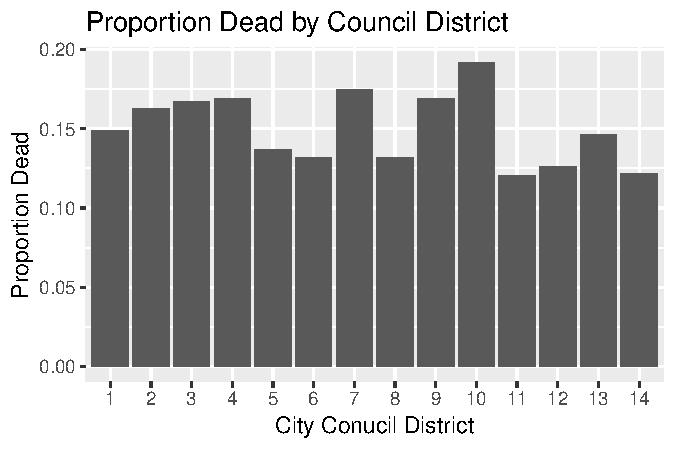
\includegraphics{Final_Report_files/figure-latex/unnamed-chunk-2-1.pdf}

\paragraph{EDA Results: Dog and Cat
Differences}\label{eda-results-dog-and-cat-differences}

\paragraph{EDA Results: Time Till Death for
Dogs}\label{eda-results-time-till-death-for-dogs}

When invesitgating the ammoint of time that dogs spend in the animal
shelter before dying or having another outcome we noticed that pitbulls
as mentioned before die much more often, but the probability of
surviving decreases faster for pitbulls than for non pitbulls.

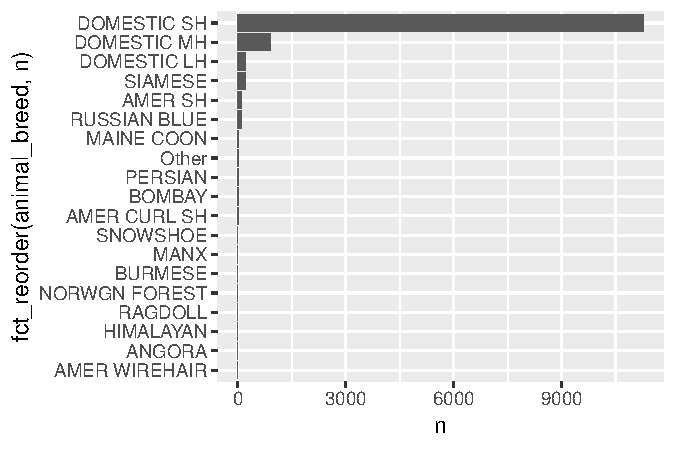
\includegraphics{Final_Report_files/figure-latex/unnamed-chunk-4-1.pdf}

\paragraph{Binomial Models for Dog
Outcomes}\label{binomial-models-for-dog-outcomes}

\begin{table}[H] \centering 
  \caption{Modeling Dog Outcomes in Dallas Animal Shelters} 
  \label{} 
\begin{tabular}{@{\extracolsep{5pt}}lD{.}{.}{-3} D{.}{.}{-3} D{.}{.}{-3} } 
\\[-1.8ex]\hline 
\hline \\[-1.8ex] 
 & \multicolumn{3}{c}{\textit{Dependent variable:}} \\ 
\cline{2-4} 
\\[-1.8ex] & \multicolumn{3}{c}{Proportion of dogs who died} \\ 
\\[-1.8ex] & \multicolumn{1}{c}{(1)} & \multicolumn{1}{c}{(2)} & \multicolumn{1}{c}{(3)}\\ 
\hline \\[-1.8ex] 
 Intercept & 0.116^{***} & 0.111^{***} & 0.552^{***} \\ 
  & \multicolumn{1}{c}{(0.069$, $0.186)} & \multicolumn{1}{c}{(0.069$, $0.170)} & \multicolumn{1}{c}{(0.454$, $0.669)} \\ 
  & & & \\ 
 Pitbull & 3.440^{***} & 3.424^{***} & 3.489^{***} \\ 
  & \multicolumn{1}{c}{(1.795$, $6.557)} & \multicolumn{1}{c}{(1.905$, $6.130)} & \multicolumn{1}{c}{(3.022$, $4.027)} \\ 
  & & & \\ 
 Scannable Chip & 0.789 & 0.799 & 0.781^{***} \\ 
  & \multicolumn{1}{c}{(0.377$, $1.566)} & \multicolumn{1}{c}{(0.412$, $1.483)} & \multicolumn{1}{c}{(0.667$, $0.911)} \\ 
  & & & \\ 
 Summer Outcome & 1.461 & 1.447 & 1.478^{***} \\ 
  & \multicolumn{1}{c}{(0.725$, $2.852)} & \multicolumn{1}{c}{(0.771$, $2.649)} & \multicolumn{1}{c}{(1.271$, $1.718)} \\ 
  & & & \\ 
 Contagious &  & 7.286^{**} & 3.975^{***} \\ 
  &  & \multicolumn{1}{c}{(1.324$, $44.137)} & \multicolumn{1}{c}{(2.568$, $6.168)} \\ 
  & & & \\ 
 Treatable At Intake &  &  & 0.161^{***} \\ 
  &  &  & \multicolumn{1}{c}{(0.133$, $0.196)} \\ 
  & & & \\ 
\hline \\[-1.8ex] 
Overdisperson Parameter & 139.72 & 111.46 & 6.27 \\ 
Nested F Test &  & F: 5.1142^* & F: 313.62^{***} \\ 
\hline 
\hline \\[-1.8ex] 
\textit{Note:}  & \multicolumn{3}{r}{$^{*}$p$<$0.1; $^{**}$p$<$0.05; $^{***}$p$<$0.01} \\ 
\end{tabular} 
\end{table}

We see in Table 3 that all of our models have variable estimates that
are significant including Model 3 which accounted for whether or not an
animal was deemed ``treatable'' at the time of intake. Further, by two F
tests we see each of our models is an improvement on the one before it
(Model 1 \(\rightarrow\) Model 2: F = 5.1141, p-value = 0.031) (Model 2
\(\rightarrow\) Model 3: F = 313.62, p-value
\textless{}\textless{}\textless{} .05).

Procceding with model 3 as our best model of dog outcomes from the
animal shelter, we glean several insights about the relationships
between certain characteristics of dogs and those animal's outcomes from
the shelter. For instance, if a dog is a pitbull, we expect it's odds of
leaving the animal shelter dead increase by 348\%, after controlling for
chip status, season, and intake condition. Further, if a dog is a
pitbull we are 95\% confident that the true increase in odds of death at
outcome is between 302\% and 402\%. Yikes! On the other hand, if a dog
comes into the shelter with a scannable chip, we expect the animals odds
of dying within the shelter system to drop by about 22\%, after
controlling for pitbull, season, and intake condition. Interestingly
enough, if a dog has its outcome in the summer, the odds of that outcome
being death are about 47\% higher, controlling for breed, chip status,
and intake condition.

\paragraph{Multilevel Model for Dog
Outcomes}\label{multilevel-model-for-dog-outcomes}

During our EDA we found that there was a difference in deaths between
city council districts this made us suspect that the guidelines within
each city coucil district might be different and that there might be
correlation within city council district. To account for this potential
correlation we used a multilevel logistic regression model.

Our model has two levels,

\begin{itemize}
\tightlist
\item
  Level 1
\end{itemize}

\[log(\frac{p_{ij}}{1-p_{ij}})=a_i+b_i*summer_{ij}+c_i*pitbull_{ij}+d_i*chipstatus_{ij}\]

\begin{itemize}
\tightlist
\item
  Level 2

  \begin{eqnarray*}  
    a_i&=\alpha_0+u_i\\
    b_i&=\beta_0+v_i\\
    c_i&=\gamma_0+w_i\\
    d_i&=\delta_0+x_i.
  \end{eqnarray*}
\end{itemize}

The variance components are described by:

\[
\begin{bmatrix} u_i \\ v_i \\ w_i\\ x_i \end{bmatrix}=N\begin{pmatrix} \begin{bmatrix} 0 \\ 0 \\ 0 \\ 0 \end{bmatrix}, \begin{bmatrix} \sigma_u^2 & & & \\ \sigma_{uv} & \sigma_v^2 & & \\ \sigma_{uvw} &\sigma_{vw} & \sigma_w^2 & \\ \sigma_{uvwx} & \sigma{vwx} & \sigma_{wx} & \sigma_x^2 \end{bmatrix} \end{pmatrix}
\]

It is important to note that the odds of a pitbull dying in the animal
shelter are 3.42 times higher than for non pitbulls accounting for
season, chip status, and intake condition, see table 4. As expected, the
odds of a contagious dog dying at the animal shelter are 3.96 time
higher than a non contagious dog accounting for whether the dog is
treatable, the season, chip status and pitbull. Also, unsuprisingly if a
dog enters the animal shelter with a treatable intake the odds of dying
in the animal shelter decrease by 84\% controlling for whether the dog
is contagious on intake, the season, and chip status.

\begin{table}[H] \centering 
  \caption{Modeling Dog Deaths in Animal Shelters using Multilevel Logistic Regression} 
  \label{} 
\begin{tabular}{@{\extracolsep{5pt}}lD{.}{.}{-3} } 
\\[-1.8ex]\hline 
\hline \\[-1.8ex] 
 & \multicolumn{1}{c}{\textit{Dependent variable:}} \\ 
\cline{2-2} 
\\[-1.8ex] & \multicolumn{1}{c}{Proportion of dogs who died} \\ 
\hline \\[-1.8ex] 
 Intercept & 3.474^{***} \\ 
  & \multicolumn{1}{c}{(3.280$, $3.680)} \\ 
  & \\ 
 Pitbull & 0.795^{***} \\ 
  & \multicolumn{1}{c}{(0.746$, $0.847)} \\ 
  & \\ 
 Scannable Chip & 1.483^{***} \\ 
  & \multicolumn{1}{c}{(1.396$, $1.575)} \\ 
  & \\ 
 Summer Outcome & 3.964^{***} \\ 
  & \multicolumn{1}{c}{(3.325$, $4.724)} \\ 
  & \\ 
 Contagious & 0.159^{***} \\ 
  & \multicolumn{1}{c}{(0.147$, $0.172)} \\ 
  & \\ 
 Treatable At Intake & 0.549^{***} \\ 
  & \multicolumn{1}{c}{(0.496$, $0.607)} \\ 
  & \\ 
\hline \\[-1.8ex] 
Observations & \multicolumn{1}{c}{45,098} \\ 
Log Likelihood & \multicolumn{1}{c}{-16,733.970} \\ 
Akaike Inf. Crit. & \multicolumn{1}{c}{33,481.950} \\ 
Bayesian Inf. Crit. & \multicolumn{1}{c}{33,542.970} \\ 
\hline 
\hline \\[-1.8ex] 
\textit{Note:}  & \multicolumn{1}{r}{$^{*}$p$<$0.1; $^{**}$p$<$0.05; $^{***}$p$<$0.01} \\ 
\end{tabular} 
\end{table}

\paragraph{Modeling Dog and Cat
Differences}\label{modeling-dog-and-cat-differences}

In our modeling of Dog and Cat differences we used used binomial
regression. To model this we considered the following model:

\[log(\frac{p_{i}}{1-p_{i}})=\beta_0+\beta_1 DogYN + \beta_i(Confounder_i)\]

We considered several models with different confounders controled for
based on findings in the literature and our EDA. We were not able to
find any significant difference in the odds of death between dogs and
cat. We conclude that there is not evidence of a significant difference
between dogs and cats in odds of dying in an animal shelter after
accounting for chip\_status, season of outcome, and intake condition.
These models can be found in the Dog Cat portion of our appendix.

\paragraph{Modeling Time Till Death for
Pitbulls}\label{modeling-time-till-death-for-pitbulls}

We approached this task by using cox proportional hazards. We wanted to
control for chip\_status and summer, but the proportional hazards
assumption was no longer met when we added these confounding variables
to our model. To get around this, we subset our data into 4 smaller
datasets, one where it was the summer and all the animals had a chip,
one where it was not the summer and all the animals had chips, one where
it was summer and none of the animals had chips, and one where it was
not the summer and the animals did not have chips. For each of our 4
datasets we fit the following model:

\[h(t)=h_0(t)*e^{b_1*Pitbull}\].

We found that in all 4 subsets of the data the coefficient for pitbull
is significant. The hazard ratio ranged from 1.69 in the subset where it
is not the summer and all the animals have chips to 1.94 in the not
summer and all animals do not have a chip dataset. In laymens terms this
means that on average at any time during an animals stay at the animal
shelter 1.69 to 1.94 times as many pitbulls have died as non pitbulls.

\begin{table}[H] \centering 
  \caption{Results of Stratified Cox Proportional Hazards Survival Analysis} 
  \label{} 
\begin{tabular}{@{\extracolsep{5pt}}lD{.}{.}{-3} D{.}{.}{-3} D{.}{.}{-3} D{.}{.}{-3} } 
\\[-1.8ex]\hline 
\hline \\[-1.8ex] 
 & \multicolumn{4}{c}{\textit{Dependent variable:}} \\ 
\cline{2-5} 
\\[-1.8ex] & \multicolumn{4}{c}{Time Spent in Animal Shelter Prior to Death} \\ 
 & \multicolumn{1}{c}{Summer and Chip} & \multicolumn{1}{c}{Summer and No Chip} & \multicolumn{1}{c}{Not Summer and Chip} & \multicolumn{1}{c}{Neither Summer or Chip} \\ 
\hline \\[-1.8ex] 
 pitbull & 1.698^{***} & 1.717^{***} & 1.694^{***} & 1.941^{***} \\ 
  & \multicolumn{1}{c}{(1.431$, $2.016)} & \multicolumn{1}{c}{(1.553$, $1.897)} & \multicolumn{1}{c}{(1.509$, $1.902)} & \multicolumn{1}{c}{(1.509$, $1.902)} \\ 
  & & & & \\ 
\hline \\[-1.8ex] 
Observations & \multicolumn{1}{c}{3,310} & \multicolumn{1}{c}{8,376} & \multicolumn{1}{c}{10,207} & \multicolumn{1}{c}{22,777} \\ 
LR Test (df = 1) & \multicolumn{1}{c}{35.288$^{***}$} & \multicolumn{1}{c}{108.543$^{***}$} & \multicolumn{1}{c}{76.212$^{***}$} & \multicolumn{1}{c}{343.664$^{***}$} \\ 
\hline 
\hline \\[-1.8ex] 
\textit{Note:}  & \multicolumn{4}{r}{$^{*}$p$<$0.1; $^{**}$p$<$0.05; $^{***}$p$<$0.01} \\ 
\end{tabular} 
\end{table}

\subsection{Discussion}\label{discussion}

\begin{itemize}
\item
  Begin with an accurate summary statement; describe how the results
  help answer your research questions and what was most interesting from
  your analysis. In fact, the first paragraph of the Discussion is very
  important -- in professional journals, it is often the first and
  sometimes the only paragraph that is read in a paper. After the first
  sentence highlights primary results, the remainder of the first
  paragraph might compare your results to others in the literature or
  include interesting secondary results.
\item
  Discuss possible implications of the results in the context of the
  research question.
\item
  Make a statement regarding potential confounding variables in your
  study
\item
  Make a statement about the generalizability of your results. Don't
  give generic statements of possible causation and generalizability,
  but thoughtfully discuss relevant issues -- confounding variables,
  representativeness of the sample, etc.
\end{itemize}

Conclusions about animal outcomes of animals in shelters from this
report can only be extended to the city of Dallas. While our sample size
is totally representative for this population, we cannot account for
differences that would be encountered in other municipalities, say
higher adoption rates or less stigma against certain breeds of dog.
Further, we cannot be sure that the trends observed in this paper will
continue into the future. Anti-pitbull advocacy groups like
\href{https://www.nationalpitbullvictimawareness.org/}{National Pitbull
Victims Awareness} and pro-pitbull advocacy groups like
\href{http://love-a-bull.org/resources/statistics-pit-bull-bites-community-safety/}{Love-a-Bull}
are at odds trying to sway public opinion and policy reguarding the
handling of pitbulls in animal shelters. If changes in public
percecption of pitbulls or the policy that surrounds them changes, our
model will lose it's generalizability to Dallas.

\begin{itemize}
\tightlist
\item
  Identify any limitations of your study. Discuss the potential impact
  of such limitations on the conclusions.
\end{itemize}

One limitation of our study is that we do not know what happens to
animals after they have been transferred out of the animal shelter. In
our analysis we have viewed this outcome as a live outcome, but for all
we know these animals could go on to another shelter where they are
euthanized. Depending on the validity of our assumption, we could be
adding some bias to our conclusions. Additionally, there is not
consistant infomration on the criteria used by shelters to evaluate
animals intake conditions. We look for key words that indicated the
health of the animal. However we are not sure how consistant these
evaluations are across all Dallas animal shelters.

\begin{itemize}
\item
  Identify strengths and weaknesses of your analysis.
\item
  Make suggestions for future research. Identify important next steps
  that a researcher could take to build on your work.
\end{itemize}

Future work could be done in Dallas to help minimize the number of
animals which need to be euthanized. By identifying specific at-risk
groups of animals, more resources could be allocated to advocating for
these animals or transfering them to other No-Kill shelters. We would
recomend any additional research to work directly with the Dallas Animal
Shelter group. By having a direct contact with the group doing data
collection, a statistician will be able to better identify pressing
issues of the group and verify certain assumptions that we have not been
able to verify.

\section{Works Cited}\label{works-cited}

\begin{enumerate}
\def\labelenumi{\arabic{enumi}.}
\tightlist
\item
  \url{https://www.aspca.org/animal-homelessness/shelter-intake-and-surrender}
\item
  \url{https://rucore.libraries.rutgers.edu/rutgers-lib/38418/PDF/1/play/}
\end{enumerate}

Patronek, G. J., \& Crowe, A. (2018). Factors Associated with High Live
Release for Dogs at a Large, Open-Admission, Municipal Shelter. Animals
: an open access journal from MDPI, 8(4), 45.
\url{doi:10.3390/ani8040045}

\href{https://www.tandfonline.com/doi/abs/10.1207/S15327604JAWS0501_3}{Lepper,
M., Kass, P. H., \& Hart, L. A. (2002). Prediction of adoption versus
euthanasia among dogs and cats in a California animal shelter. Journal
of Applied Animal Welfare Science, 5(1), 29-42.}

\href{https://europepmc.org/abstract/med/9713528}{Posage, J. M.,
Bartlett, P. C., \& Thomas, D. K. (1998). Determining factors for
successful adoption of dogs from an animal shelter. Journal of the
American Veterinary Medical Association, 213(4), 478-482.}

\href{https://www.tandfonline.com/doi/abs/10.1080/10888705.2014.982796}{Lampe,
R., \& Witte, T. H. (2015). Speed of dog adoption: Impact of online
photo traits. Journal of applied animal welfare science, 18(4),
343-354.}

\begin{enumerate}
\def\labelenumi{\arabic{enumi}.}
\setcounter{enumi}{4}
\tightlist
\item
  Annotated Appendix
\end{enumerate}

\begin{itemize}
\tightlist
\item
  Tables and figures that are informative but were not referenced
  specifically in the main report. Include a short annotation -- one or
  two sentences on what they show.
\item
  R scripts and output (annotated) so that I can trace how you
  constructed your final data set, what models you ran to produce the
  results quoted in your report, and what intermediate models you also
  considered.
\item
  Description of statistical modeling steps that were not included in
  the main body of your report. Possible entries here include: How you
  handled missing data. Evaluation of assumptions. Outlier analysis and
  how you decided to deal with any outliers along with rationale for
  your decision. Describe hypotheses testing you performed during model
  building and how you decided on the explanatory variables you
  ultimately included in your final model. Assessment of the final
  model.
\item
  How you went from the model output in R to interpretations in your
  report (e.g.~exponentiate coefficients, then take inverse)
\item
  Anticipate questions someone might have after reading your report, and
  make sure those questions can be answered with information in the
  appendix.
\item
  A citation for each reference article (in APA format or something
  similar) you included in your proposal. Also include a link, if
  appropriate. Remember that you must have the entire paper and not just
  an abstract, and at least two must be from peer-reviewed journals.
\end{itemize}

\subsubsection{Dogs vs Cats}\label{dogs-vs-cats}

\begin{Shaded}
\begin{Highlighting}[]
\NormalTok{cat_dog_binom <-}\StringTok{ }\NormalTok{adoptions }\OperatorTok
\StringTok{  }\KeywordTok{filter}\NormalTok{(}\OperatorTok{!}\KeywordTok{str_detect}\NormalTok{(intake_subtype, }\StringTok{"(DEAD)|(DIED)"}\NormalTok{)) }\OperatorTok
\StringTok{  }\KeywordTok{filter}\NormalTok{(dog }\OperatorTok{==}\StringTok{ }\DecValTok{1} \OperatorTok{|}\StringTok{ }\NormalTok{cat }\OperatorTok{==}\StringTok{ }\DecValTok{1}\NormalTok{) }\OperatorTok
\StringTok{  }\KeywordTok{mutate}\NormalTok{(}\DataTypeTok{out_dead =}\NormalTok{ outcome_type }\OperatorTok\StringTok{ }\KeywordTok{c}\NormalTok{(}\StringTok{"DEAD ON ARRIVAL"}\NormalTok{, }\StringTok{"EUTHANIZED"}\NormalTok{, }\StringTok{"DIED"}\NormalTok{),}
         \DataTypeTok{summer =} \KeywordTok{ifelse}\NormalTok{(month }\OperatorTok\StringTok{ }\KeywordTok{c}\NormalTok{(}\DecValTok{5}\NormalTok{, }\DecValTok{6}\NormalTok{, }\DecValTok{7}\NormalTok{, }\DecValTok{8}\NormalTok{, }\DecValTok{9}\NormalTok{), }\DecValTok{1}\NormalTok{, }\DecValTok{0}\NormalTok{))}\OperatorTok
\StringTok{  }\KeywordTok{mutate}\NormalTok{(}\DataTypeTok{chip_status =} \KeywordTok{ifelse}\NormalTok{(chip_status}\OperatorTok{==}\StringTok{"SCAN CHIP"}\NormalTok{, }\DecValTok{1}\NormalTok{, }\DecValTok{0}\NormalTok{)) }\OperatorTok
\StringTok{  }\KeywordTok{group_by}\NormalTok{(dog, chip_status, summer, stray) }\OperatorTok
\StringTok{  }\KeywordTok{summarize}\NormalTok{(}\DataTypeTok{prop_dead =} \KeywordTok{sum}\NormalTok{(out_dead)}\OperatorTok{/}\KeywordTok{n}\NormalTok{(), }\DataTypeTok{count =} \KeywordTok{n}\NormalTok{())}

\NormalTok{####### MODEL 1: dog #########}

\NormalTok{dogcat_model1_binom <-}\StringTok{ }\KeywordTok{glm}\NormalTok{(prop_dead }\OperatorTok{~}\StringTok{ }\NormalTok{dog, }\DataTypeTok{weights =}\NormalTok{ count, }\DataTypeTok{family =}\NormalTok{ binomial, }\DataTypeTok{data =}\NormalTok{ cat_dog_binom)}

\NormalTok{dogcat_model1_quasi <-}\StringTok{ }\KeywordTok{glm}\NormalTok{(prop_dead }\OperatorTok{~}\StringTok{ }\NormalTok{dog, }\DataTypeTok{weights =}\NormalTok{ count, }\DataTypeTok{family =}\NormalTok{ quasibinomial, }\DataTypeTok{data =}\NormalTok{ cat_dog_binom)}

\KeywordTok{summary}\NormalTok{(dogcat_model1_binom)}
\end{Highlighting}
\end{Shaded}

\begin{verbatim}
## 
## Call:
## glm(formula = prop_dead ~ dog, family = binomial, data = cat_dog_binom, 
##     weights = count)
## 
## Deviance Residuals: 
##     Min       1Q   Median       3Q      Max  
## -19.837   -7.385   -2.250    4.985   15.639  
## 
## Coefficients:
##             Estimate Std. Error z value Pr(>|z|)    
## (Intercept) -1.43741    0.02199  -65.38   <2e-16 ***
## dog         -0.30509    0.02563  -11.90   <2e-16 ***
## ---
## Signif. codes:  0 '***' 0.001 '**' 0.01 '*' 0.05 '.' 0.1 ' ' 1
## 
## (Dispersion parameter for binomial family taken to be 1)
## 
##     Null deviance: 1883.0  on 17  degrees of freedom
## Residual deviance: 1745.6  on 16  degrees of freedom
## AIC: 1866
## 
## Number of Fisher Scoring iterations: 4
\end{verbatim}

\begin{Shaded}
\begin{Highlighting}[]
\KeywordTok{exp}\NormalTok{(}\KeywordTok{confint}\NormalTok{(dogcat_model1_binom))}
\end{Highlighting}
\end{Shaded}

\begin{verbatim}
## Waiting for profiling to be done...
\end{verbatim}

\begin{verbatim}
##                 2.5 %    97.5 %
## (Intercept) 0.2274800 0.2479563
## dog         0.7010303 0.7751213
\end{verbatim}

\begin{Shaded}
\begin{Highlighting}[]
\KeywordTok{summary}\NormalTok{(dogcat_model1_quasi)}
\end{Highlighting}
\end{Shaded}

\begin{verbatim}
## 
## Call:
## glm(formula = prop_dead ~ dog, family = quasibinomial, data = cat_dog_binom, 
##     weights = count)
## 
## Deviance Residuals: 
##     Min       1Q   Median       3Q      Max  
## -19.837   -7.385   -2.250    4.985   15.639  
## 
## Coefficients:
##             Estimate Std. Error t value Pr(>|t|)    
## (Intercept)  -1.4374     0.2249  -6.393 8.91e-06 ***
## dog          -0.3051     0.2621  -1.164    0.261    
## ---
## Signif. codes:  0 '***' 0.001 '**' 0.01 '*' 0.05 '.' 0.1 ' ' 1
## 
## (Dispersion parameter for quasibinomial family taken to be 104.5899)
## 
##     Null deviance: 1883.0  on 17  degrees of freedom
## Residual deviance: 1745.6  on 16  degrees of freedom
## AIC: NA
## 
## Number of Fisher Scoring iterations: 4
\end{verbatim}

\begin{Shaded}
\begin{Highlighting}[]
\KeywordTok{exp}\NormalTok{(}\KeywordTok{confint}\NormalTok{(dogcat_model1_quasi))}
\end{Highlighting}
\end{Shaded}

\begin{verbatim}
## Waiting for profiling to be done...
\end{verbatim}

\begin{verbatim}
##                 2.5 %    97.5 %
## (Intercept) 0.1495373 0.3624932
## dog         0.4457027 1.2501118
\end{verbatim}

\begin{Shaded}
\begin{Highlighting}[]
\NormalTok{####### MODEL 2: dog + summer #########}

\NormalTok{dogcat_model2_binom <-}\StringTok{ }\KeywordTok{glm}\NormalTok{(prop_dead }\OperatorTok{~}\StringTok{ }\NormalTok{dog }\OperatorTok{+}\StringTok{ }\NormalTok{summer, }\DataTypeTok{weights =}\NormalTok{ count, }\DataTypeTok{family =}\NormalTok{ binomial, }\DataTypeTok{data =}\NormalTok{ cat_dog_binom)}

\NormalTok{dogcat_model2_quasi <-}\StringTok{ }\KeywordTok{glm}\NormalTok{(prop_dead }\OperatorTok{~}\StringTok{ }\NormalTok{dog }\OperatorTok{+}\StringTok{ }\NormalTok{summer, }\DataTypeTok{weights =}\NormalTok{ count, }\DataTypeTok{family =}\NormalTok{ quasibinomial, }\DataTypeTok{data =}\NormalTok{ cat_dog_binom)}

\KeywordTok{summary}\NormalTok{(dogcat_model2_binom)}
\end{Highlighting}
\end{Shaded}

\begin{verbatim}
## 
## Call:
## glm(formula = prop_dead ~ dog + summer, family = binomial, data = cat_dog_binom, 
##     weights = count)
## 
## Deviance Residuals: 
##     Min       1Q   Median       3Q      Max  
## -17.003   -6.915   -5.412    5.530   19.155  
## 
## Coefficients:
##             Estimate Std. Error z value Pr(>|z|)    
## (Intercept) -1.61541    0.02452 -65.870   <2e-16 ***
## dog         -0.24951    0.02590  -9.632   <2e-16 ***
## summer       0.42766    0.02392  17.879   <2e-16 ***
## ---
## Signif. codes:  0 '***' 0.001 '**' 0.01 '*' 0.05 '.' 0.1 ' ' 1
## 
## (Dispersion parameter for binomial family taken to be 1)
## 
##     Null deviance: 1883.0  on 17  degrees of freedom
## Residual deviance: 1434.4  on 15  degrees of freedom
## AIC: 1556.8
## 
## Number of Fisher Scoring iterations: 4
\end{verbatim}

\begin{Shaded}
\begin{Highlighting}[]
\KeywordTok{exp}\NormalTok{(}\KeywordTok{confint}\NormalTok{(dogcat_model2_binom))}
\end{Highlighting}
\end{Shaded}

\begin{verbatim}
## Waiting for profiling to be done...
\end{verbatim}

\begin{verbatim}
##                 2.5 %    97.5 %
## (Intercept) 0.1894425 0.2085590
## dog         0.7407010 0.8198698
## summer      1.4633398 1.6071906
\end{verbatim}

\begin{Shaded}
\begin{Highlighting}[]
\KeywordTok{summary}\NormalTok{(dogcat_model2_quasi)}
\end{Highlighting}
\end{Shaded}

\begin{verbatim}
## 
## Call:
## glm(formula = prop_dead ~ dog + summer, family = quasibinomial, 
##     data = cat_dog_binom, weights = count)
## 
## Deviance Residuals: 
##     Min       1Q   Median       3Q      Max  
## -17.003   -6.915   -5.412    5.530   19.155  
## 
## Coefficients:
##             Estimate Std. Error t value Pr(>|t|)    
## (Intercept)  -1.6154     0.2344  -6.892 5.13e-06 ***
## dog          -0.2495     0.2476  -1.008    0.330    
## summer        0.4277     0.2286   1.871    0.081 .  
## ---
## Signif. codes:  0 '***' 0.001 '**' 0.01 '*' 0.05 '.' 0.1 ' ' 1
## 
## (Dispersion parameter for quasibinomial family taken to be 91.33309)
## 
##     Null deviance: 1883.0  on 17  degrees of freedom
## Residual deviance: 1434.4  on 15  degrees of freedom
## AIC: NA
## 
## Number of Fisher Scoring iterations: 4
\end{verbatim}

\begin{Shaded}
\begin{Highlighting}[]
\KeywordTok{exp}\NormalTok{(}\KeywordTok{confint}\NormalTok{(dogcat_model2_quasi))}
\end{Highlighting}
\end{Shaded}

\begin{verbatim}
## Waiting for profiling to be done...
\end{verbatim}

\begin{verbatim}
##                 2.5 %    97.5 %
## (Intercept) 0.1232172 0.3096656
## dog         0.4842912 1.2820599
## summer      0.9734565 2.3902024
\end{verbatim}

\begin{Shaded}
\begin{Highlighting}[]
\NormalTok{####### MODEL 3: dog + chip ######}

\NormalTok{dogcat_model3_binom <-}\StringTok{ }\KeywordTok{glm}\NormalTok{(prop_dead }\OperatorTok{~}\StringTok{ }\NormalTok{dog }\OperatorTok{+}\StringTok{ }\NormalTok{chip_status, }\DataTypeTok{weights =}\NormalTok{ count, }\DataTypeTok{family =}\NormalTok{ binomial, }\DataTypeTok{data =}\NormalTok{ cat_dog_binom)}

\NormalTok{dogcat_model3_quasi <-}\StringTok{ }\KeywordTok{glm}\NormalTok{(prop_dead }\OperatorTok{~}\StringTok{ }\NormalTok{dog }\OperatorTok{+}\StringTok{ }\NormalTok{chip_status, }\DataTypeTok{weights =}\NormalTok{ count, }\DataTypeTok{family =}\NormalTok{ quasibinomial, }\DataTypeTok{data =}\NormalTok{ cat_dog_binom)}

\KeywordTok{summary}\NormalTok{(dogcat_model3_binom)}
\end{Highlighting}
\end{Shaded}

\begin{verbatim}
## 
## Call:
## glm(formula = prop_dead ~ dog + chip_status, family = binomial, 
##     data = cat_dog_binom, weights = count)
## 
## Deviance Residuals: 
##      Min        1Q    Median        3Q       Max  
## -15.6677   -4.1391    0.1846   10.8318   14.4792  
## 
## Coefficients:
##             Estimate Std. Error z value Pr(>|z|)    
## (Intercept) -1.40636    0.02211 -63.599   <2e-16 ***
## dog         -0.24565    0.02620  -9.377   <2e-16 ***
## chip_status -0.29305    0.02828 -10.363   <2e-16 ***
## ---
## Signif. codes:  0 '***' 0.001 '**' 0.01 '*' 0.05 '.' 0.1 ' ' 1
## 
## (Dispersion parameter for binomial family taken to be 1)
## 
##     Null deviance: 1750.8  on 15  degrees of freedom
## Residual deviance: 1503.0  on 13  degrees of freedom
##   (2 observations deleted due to missingness)
## AIC: 1625.4
## 
## Number of Fisher Scoring iterations: 4
\end{verbatim}

\begin{Shaded}
\begin{Highlighting}[]
\KeywordTok{exp}\NormalTok{(}\KeywordTok{confint}\NormalTok{(dogcat_model3_binom))}
\end{Highlighting}
\end{Shaded}

\begin{verbatim}
## Waiting for profiling to be done...
\end{verbatim}

\begin{verbatim}
##                 2.5 %    97.5 %
## (Intercept) 0.2345951 0.2558385
## dog         0.7431337 0.8235017
## chip_status 0.7056151 0.7883420
\end{verbatim}

\begin{Shaded}
\begin{Highlighting}[]
\KeywordTok{summary}\NormalTok{(dogcat_model3_quasi)}
\end{Highlighting}
\end{Shaded}

\begin{verbatim}
## 
## Call:
## glm(formula = prop_dead ~ dog + chip_status, family = quasibinomial, 
##     data = cat_dog_binom, weights = count)
## 
## Deviance Residuals: 
##      Min        1Q    Median        3Q       Max  
## -15.6677   -4.1391    0.1846   10.8318   14.4792  
## 
## Coefficients:
##             Estimate Std. Error t value Pr(>|t|)    
## (Intercept)  -1.4064     0.2391  -5.883 5.38e-05 ***
## dog          -0.2456     0.2832  -0.867    0.401    
## chip_status  -0.2931     0.3057  -0.959    0.355    
## ---
## Signif. codes:  0 '***' 0.001 '**' 0.01 '*' 0.05 '.' 0.1 ' ' 1
## 
## (Dispersion parameter for quasibinomial family taken to be 116.867)
## 
##     Null deviance: 1750.8  on 15  degrees of freedom
## Residual deviance: 1503.0  on 13  degrees of freedom
##   (2 observations deleted due to missingness)
## AIC: NA
## 
## Number of Fisher Scoring iterations: 4
\end{verbatim}

\begin{Shaded}
\begin{Highlighting}[]
\KeywordTok{exp}\NormalTok{(}\KeywordTok{confint}\NormalTok{(dogcat_model3_quasi))}
\end{Highlighting}
\end{Shaded}

\begin{verbatim}
## Waiting for profiling to be done...
\end{verbatim}

\begin{verbatim}
##                 2.5 %    97.5 %
## (Intercept) 0.1496550 0.3838132
## dog         0.4540004 1.3839138
## chip_status 0.3987708 1.3312323
\end{verbatim}

\begin{Shaded}
\begin{Highlighting}[]
\NormalTok{####### MODEL 4: summer + dog + summer:dog ######}

\NormalTok{dogcat_model4_binom <-}\StringTok{ }\KeywordTok{glm}\NormalTok{(prop_dead }\OperatorTok{~}\StringTok{ }\NormalTok{summer}\OperatorTok{+}\NormalTok{dog}\OperatorTok{+}\StringTok{ }\NormalTok{summer}\OperatorTok{:}\NormalTok{dog, }\DataTypeTok{weights =}\NormalTok{ count, }\DataTypeTok{family =}\NormalTok{ binomial, }\DataTypeTok{data =}\NormalTok{ cat_dog_binom)}

\NormalTok{dogcat_model4_quasi <-}\StringTok{ }\KeywordTok{glm}\NormalTok{(prop_dead }\OperatorTok{~}\StringTok{ }\NormalTok{summer}\OperatorTok{+}\NormalTok{dog}\OperatorTok{+}\StringTok{ }\NormalTok{summer}\OperatorTok{:}\NormalTok{dog, }\DataTypeTok{weights =}\NormalTok{ count, }\DataTypeTok{family =}\NormalTok{ quasibinomial, }\DataTypeTok{data =}\NormalTok{ cat_dog_binom)}

\KeywordTok{summary}\NormalTok{(dogcat_model4_binom)}
\end{Highlighting}
\end{Shaded}

\begin{verbatim}
## 
## Call:
## glm(formula = prop_dead ~ summer + dog + summer:dog, family = binomial, 
##     data = cat_dog_binom, weights = count)
## 
## Deviance Residuals: 
##     Min       1Q   Median       3Q      Max  
## -17.392   -7.749   -4.789    6.527   18.670  
## 
## Coefficients:
##             Estimate Std. Error z value Pr(>|z|)    
## (Intercept) -1.67600    0.03030 -55.313  < 2e-16 ***
## summer       0.56018    0.04434  12.634  < 2e-16 ***
## dog         -0.17185    0.03420  -5.024 5.05e-07 ***
## summer:dog  -0.18718    0.05275  -3.549 0.000387 ***
## ---
## Signif. codes:  0 '***' 0.001 '**' 0.01 '*' 0.05 '.' 0.1 ' ' 1
## 
## (Dispersion parameter for binomial family taken to be 1)
## 
##     Null deviance: 1883.0  on 17  degrees of freedom
## Residual deviance: 1421.8  on 14  degrees of freedom
## AIC: 1546.2
## 
## Number of Fisher Scoring iterations: 4
\end{verbatim}

\begin{Shaded}
\begin{Highlighting}[]
\KeywordTok{exp}\NormalTok{(}\KeywordTok{confint}\NormalTok{(dogcat_model4_binom))}
\end{Highlighting}
\end{Shaded}

\begin{verbatim}
## Waiting for profiling to be done...
\end{verbatim}

\begin{verbatim}
##                 2.5 %    97.5 %
## (Intercept) 0.1762591 0.1984903
## summer      1.6052408 1.9099840
## dog         0.7877336 0.9007624
## summer:dog  0.7478053 0.9195843
\end{verbatim}

\begin{Shaded}
\begin{Highlighting}[]
\KeywordTok{summary}\NormalTok{(dogcat_model4_quasi)}
\end{Highlighting}
\end{Shaded}

\begin{verbatim}
## 
## Call:
## glm(formula = prop_dead ~ summer + dog + summer:dog, family = quasibinomial, 
##     data = cat_dog_binom, weights = count)
## 
## Deviance Residuals: 
##     Min       1Q   Median       3Q      Max  
## -17.392   -7.749   -4.789    6.527   18.670  
## 
## Coefficients:
##             Estimate Std. Error t value Pr(>|t|)    
## (Intercept)  -1.6760     0.2978  -5.628 6.23e-05 ***
## summer        0.5602     0.4358   1.285    0.220    
## dog          -0.1718     0.3362  -0.511    0.617    
## summer:dog   -0.1872     0.5185  -0.361    0.723    
## ---
## Signif. codes:  0 '***' 0.001 '**' 0.01 '*' 0.05 '.' 0.1 ' ' 1
## 
## (Dispersion parameter for quasibinomial family taken to be 96.60753)
## 
##     Null deviance: 1883.0  on 17  degrees of freedom
## Residual deviance: 1421.8  on 14  degrees of freedom
## AIC: NA
## 
## Number of Fisher Scoring iterations: 4
\end{verbatim}

\begin{Shaded}
\begin{Highlighting}[]
\KeywordTok{exp}\NormalTok{(}\KeywordTok{confint}\NormalTok{(dogcat_model4_quasi))}
\end{Highlighting}
\end{Shaded}

\begin{verbatim}
## Waiting for profiling to be done...
\end{verbatim}

\begin{verbatim}
##                  2.5 %   97.5 %
## (Intercept) 0.09987833 0.324086
## summer      0.74071253 4.144038
## dog         0.44621757 1.682512
## summer:dog  0.29772816 2.292399
\end{verbatim}

\begin{Shaded}
\begin{Highlighting}[]
\NormalTok{####### MODEL 5: stray ######}

\NormalTok{dogcat_model5_binom <-}\StringTok{ }\KeywordTok{glm}\NormalTok{(prop_dead }\OperatorTok{~}\StringTok{ }\NormalTok{dog }\OperatorTok{+}\StringTok{ }\NormalTok{stray, }\DataTypeTok{weights =}\NormalTok{ count, }\DataTypeTok{family =}\NormalTok{ binomial, }\DataTypeTok{data =}\NormalTok{ cat_dog_binom)}

\NormalTok{dogcat_model5_quasi <-}\StringTok{ }\KeywordTok{glm}\NormalTok{(prop_dead }\OperatorTok{~}\StringTok{ }\NormalTok{dog }\OperatorTok{+}\StringTok{ }\NormalTok{stray, }\DataTypeTok{weights =}\NormalTok{ count, }\DataTypeTok{family =}\NormalTok{ quasibinomial, }\DataTypeTok{data =}\NormalTok{ cat_dog_binom)}

\KeywordTok{summary}\NormalTok{(dogcat_model5_binom)}
\end{Highlighting}
\end{Shaded}

\begin{verbatim}
## 
## Call:
## glm(formula = prop_dead ~ dog + stray, family = binomial, data = cat_dog_binom, 
##     weights = count)
## 
## Deviance Residuals: 
##     Min       1Q   Median       3Q      Max  
## -16.892   -6.265   -2.337    5.256   18.556  
## 
## Coefficients:
##             Estimate Std. Error z value Pr(>|z|)    
## (Intercept) -1.23402    0.02551  -48.38   <2e-16 ***
## dog         -0.28633    0.02571  -11.13   <2e-16 ***
## stray       -0.34943    0.02308  -15.14   <2e-16 ***
## ---
## Signif. codes:  0 '***' 0.001 '**' 0.01 '*' 0.05 '.' 0.1 ' ' 1
## 
## (Dispersion parameter for binomial family taken to be 1)
## 
##     Null deviance: 1883.0  on 17  degrees of freedom
## Residual deviance: 1519.7  on 15  degrees of freedom
## AIC: 1642.1
## 
## Number of Fisher Scoring iterations: 4
\end{verbatim}

\begin{Shaded}
\begin{Highlighting}[]
\KeywordTok{exp}\NormalTok{(}\KeywordTok{confint}\NormalTok{(dogcat_model5_binom))}
\end{Highlighting}
\end{Shaded}

\begin{verbatim}
## Waiting for profiling to be done...
\end{verbatim}

\begin{verbatim}
##                 2.5 %    97.5 %
## (Intercept) 0.2768768 0.3059909
## dog         0.7141890 0.7899317
## stray       0.6739322 0.7377448
\end{verbatim}

\begin{Shaded}
\begin{Highlighting}[]
\KeywordTok{summary}\NormalTok{(dogcat_model5_quasi)}
\end{Highlighting}
\end{Shaded}

\begin{verbatim}
## 
## Call:
## glm(formula = prop_dead ~ dog + stray, family = quasibinomial, 
##     data = cat_dog_binom, weights = count)
## 
## Deviance Residuals: 
##     Min       1Q   Median       3Q      Max  
## -16.892   -6.265   -2.337    5.256   18.556  
## 
## Coefficients:
##             Estimate Std. Error t value Pr(>|t|)    
## (Intercept)  -1.2340     0.2487  -4.961 0.000171 ***
## dog          -0.2863     0.2508  -1.142 0.271435    
## stray        -0.3494     0.2251  -1.553 0.141379    
## ---
## Signif. codes:  0 '***' 0.001 '**' 0.01 '*' 0.05 '.' 0.1 ' ' 1
## 
## (Dispersion parameter for quasibinomial family taken to be 95.10904)
## 
##     Null deviance: 1883.0  on 17  degrees of freedom
## Residual deviance: 1519.7  on 15  degrees of freedom
## AIC: NA
## 
## Number of Fisher Scoring iterations: 4
\end{verbatim}

\begin{Shaded}
\begin{Highlighting}[]
\KeywordTok{exp}\NormalTok{(}\KeywordTok{confint}\NormalTok{(dogcat_model5_quasi))}
\end{Highlighting}
\end{Shaded}

\begin{verbatim}
## Waiting for profiling to be done...
\end{verbatim}

\begin{verbatim}
##                 2.5 %    97.5 %
## (Intercept) 0.1755655 0.4670297
## dog         0.4639650 1.2440641
## stray       0.4546178 1.1008372
\end{verbatim}


\end{document}
